% Capítulo 4: fila circular em vetor de 6 posições (início = 4, fim = 1).
\documentclass[border=4pt]{standalone}
\usepackage[utf8]{inputenc}
\usepackage[T1]{fontenc}
% Estilo comum das figuras de listas (incluído pelas figuras dos capítulos 3 e 4).
\usepackage{tikz}
\usetikzlibrary{arrows.meta, positioning, shapes.multipart, calc}
\definecolor{navy}{RGB}{23,45,80}
\definecolor{laranja}{RGB}{250,110,29}
\definecolor{cinzalogo}{RGB}{107,114,126}
\tikzset{
  no/.style={rectangle split, rectangle split horizontal, rectangle split parts=2,
             draw=navy, line width=0.9pt, minimum height=7mm,
             rectangle split part fill={laranja!15, white}, font=\sffamily\small},
  no3/.style={rectangle split, rectangle split horizontal, rectangle split parts=3,
              draw=navy, line width=0.9pt, minimum height=7mm,
              rectangle split part fill={white, laranja!15, white}, font=\sffamily\small},
  seta/.style={-{Stealth[length=2.2mm]}, navy, line width=0.9pt},
  setanova/.style={-{Stealth[length=2.2mm]}, laranja, line width=1.3pt},
  rotulo/.style={font=\sffamily\small\bfseries, text=navy},
  nulo/.style={font=\sffamily\scriptsize, text=cinzalogo},
  passo/.style={font=\sffamily\small, text=cinzalogo, anchor=west},
  legenda/.style={font=\sffamily\scriptsize, text=cinzalogo},
}
% seta que sai do meio da caixa do ponteiro (última parte do nó), na horizontal
\newcommand{\liga}[3][seta]{\draw[#1] ([xshift=-2.3mm]#2.east) -- #3;}

\tikzset{
  casa/.style={draw=navy, line width=0.9pt, minimum width=11mm, minimum height=8mm, font=\sffamily\small},
  cheia/.style={casa, fill=laranja!15},
  indice/.style={font=\sffamily\scriptsize, text=cinzalogo},
}
\begin{document}
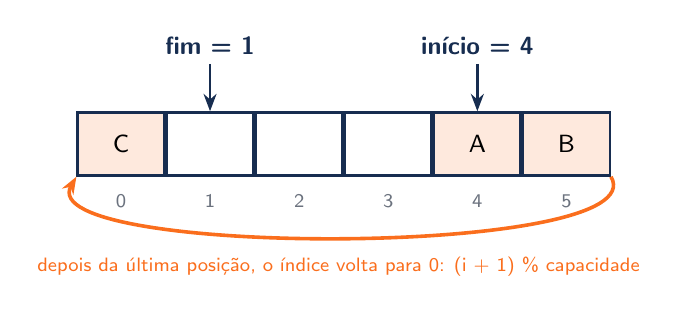
\begin{tikzpicture}
  % vetor de 6 posições: ocupadas 4, 5, 0 (ordem de saída: 4 -> 5 -> 0)
  \node[cheia] (v0) at (0,0) {C};
  \node[casa, right=0mm of v0] (v1) {};
  \node[casa, right=0mm of v1] (v2) {};
  \node[casa, right=0mm of v2] (v3) {};
  \node[cheia, right=0mm of v3] (v4) {A};
  \node[cheia, right=0mm of v4] (v5) {B};
  \foreach \i in {0,...,5} { \node[indice, below=1mm of v\i] {\i}; }
  \node[rotulo, above=6mm of v4] (ini) {início = 4};
  \node[rotulo, above=6mm of v1] (fim) {fim = 1};
  \draw[seta] (ini) -- (v4.north);
  \draw[seta] (fim) -- (v1.north);
  \draw[setanova] (v5.south east) to[out=-60, in=-120, looseness=0.45] (v0.south west);
  \node[legenda, text=laranja, below=9mm of v2, xshift=5mm]
    {depois da última posição, o índice volta para 0: (i + 1) \% capacidade};
\end{tikzpicture}
\end{document}
